از دیدگاه مهندسی نیازمند‌ی نرم‌افزار\LTRfootnote{software requirement engineering}، مجموعه‌ی نیازمندی‌های یک سیستم نرم‌افزاری را می‌توان در دو دسته‌ی کلی {\it کارکردی\LTRfootnote{functional}} و {\it غیرکارکردی\LTRfootnote{non-functional}} طبقه‌بندی نمود \cite{Greene05}. مطابق این طبقه‌بندی، نیازهای کارکردی عملکرد درست نرم‌افزار را از دید کاربران تعیین می‌کنند. در دید غیرکارکردی نیز به چگونگی عملکرد سیستم و شرایط آن می‌پردازد و در واقع مشخص می‌کند که سیستم با چه کیفیتی در محیط اجرای خود فعالیت خواهد نمود. در ادامه‌ی این متن تنها به بررسی نیازهای کارکردی نرم‌افزار خواهیم پرداخت.

برای اطمینان از صحت پیاده‌سازی نیازمندی‌های نرم‌افزار در متن پیاده‌سازی شده روش‌های مختلفی پیشنهاد شده و مورد استفاده قرار می‌گیرد. برای مثال \emph{آزمون نرم‌افزار}\LTRfootnote{software testing}، دسته‌ای از روش‌ها را برای بازرسی \gls*{مطابقت}\LTRfootnote{conformance} متن برنامه\LTRfootnote{source code} و نیازهای سیستم معرفی می‌کند. در روش‌های آزمون از اِعمال \glspl*{مورد آزمون}\LTRfootnote{test cases} بر سیستم تحت آزمون برای سنجش این مطابقت استفاده می‌شود. هر مورد آزمون عبارت است از ترتیبی تعریف شده از عملیات بر روی سیستم و هم‌چنین نتیجه‌ای که در قبال این عملیات از سیستم مورد انتظار است \cite{ammann08}.

یک طبقه‌بندی شناخته شده، روش‌های آزمون نرم‌افزار را به دو دسته‌ی کلی \emph{آزمون کارکردی} و \emph{آزمون ساختاری} تقسیم می‌کند \cite{Jorgensen08}، اگرچه این تقسیم‌بندی کاملاً استاندارد و همه‌گیر نیست. آزمون کارکردی (که معمولاً با نام آزمون جعبه-سیاه\LTRfootnote{black-box testing} شناخته می‌شود) بدون اطلاع از نحوه‌ی پیاده‌سازی سیستم‌ انجام شده و تنها به توصیف‌های سطح بالای سیستم متکی است. در مقابل ایده‌ی آزمون کارکردی، آزمون ساختاری قرار دارد (که با نام آزمون جعبه-سفید\LTRfootnote{white-box testing} نیز شناخته‌ می‌شود). در این ایده، از ساختار داخلی کد و اطلاعات مربوط به نحوه‌ی پیاده‌سازی استفاده شده و تلاش می‌شود تمامی حالت‌هایی که درون متنِ برنامه‌ی پیاده شده است مورد بررسی قرار گیرد.

از جمله‌ی روش‌های جعبه‌-سیاه شناخته شده، \emph{آزمون مبتنی بر مدل}\LTRfootnote{model-based testing}\cite{Ap97modelbased} است. آزمون مبتنی بر مدل تلاش می‌کند تا با مدل‌سازی رفتار سیستم (که از آن  به عنوان توصیف\LTRfootnote{specification} سیستم یاد می‌شود) و تحلیل آن، به طور خودکار به تولید موارد آزمون پرداخته و علاوه بر آن مراحل اجرا و بررسی نتایج آزمون را نیز به صورت خودکار انجام دهد. به این ترتیب، در آزمون مبتنی بر مدل مهم‌ترین فعالیت در طراحی آزمون‌ها، ساختن مدلی از  رفتار سیستم و تعیین چگونگی ارتباط آن با سیستم اصلی است. با توجه به خودکار بودن مراحل تولید موارد آزمون، لازم است نمادگذاری‌های به کار رفته برای مدل‌سازی با اتکا بر \glspl*{روش صوری}\LTRfootnote{formal methods} طراحی شوند تا امکان پردازش خودکار آن‌ها فراهم شود.

استفاده از ایده‌ی آزمون مبتنی بر مدل خصوصاً در مورد سیستم‌های با توصیف پیچیده بسیار مفید خواهد بود. در این سیستم‌ها، به دلیل تعدّد عملکرد‌های سیستم، برای اطمینان از صحت کارکرد آن‌ها باید تعداد زیادی مورد آزمون طراحی نمود. واضح است که در صورت استفاده از روش‌های متداول آزمون، نگه‌داری این مجموعه‌ی آزمون دشوار خواهد بود، زیرا به وجود آمدن تغییراتی در متن برنامه ممکن است تغییرات زیادی در آزمون‌های طراحی شده را طلب کند. در مقابل در  روش‌های آزمون مبتنی بر مدل با بروز تغییرات در ساختار و متن برنامه‌ی تحت آزمون تنها کافی است مدل توصیف‌کننده سیستم، تغییر کند، در این صورت موارد آزمون مجدداً با استفاده از این مدل جدید به صورت خودکار تولید خواهند شد. مزیت دیگر استفاده از روش‌های آزمون مبتنی بر مدل، خصوصاً برای سیستم‌های با رفتارهای نسبتاً پیچیده، اطمینان از فراموش نشدن برخی آزمون‌های مهم است. در روش‌های متداول آزمون، به دلیل دستی بودن فرآیند طراحی آزمون‌ها و نیز تعدد آن‌ها، ممکن است برخی از آن‌ها (به خاطر احتمال بروز خطای انسانی) از قلم بیفتند که این احتمال در روش‌های آزمون مبتنی بر مدل (با توجه به سیستماتیک بودن مراحل تولید موارد آزمون) به طور کلی از بین می‌رود.

بسته به نمادگذاری به کار رفته در مدل‌سازی و نیز روش تولید موارد آزمون از روی این توصیف‌ها، روش‌های متفاوتی برای آزمون مبتنی بر مدل ارائه شده است. در این‌جا بر گونه‌ی خاصی از آزمون مبتنی بر مدل به نام \emph{آی‌او‌کو}\LTRfootnote{ioco}\cite{tret96} تمرکز می‌کنیم. در این روش از نمادگذاری \emph{ماشین‌های گذار}\LTRfootnote{transition systems} برای توصیف رفتار سیستم استفاده می‌شود. 

در گونه‌های امروزی آی‌او‌کو، موارد آزمون به صورت در-لحظه\LTRfootnote{on-the-fly} تولید می‌شوند. به عبارت دیگر آزمون‌گر مبتنی بر مدل در زمان اجرای آزمون‌ها و با توجه به الگوریتم، یک مورد آزمون تولید و بر روی سیستم اعمال می‌کند. هم‌چنین، آزمون‌گر خروجی‌های سیستم را مشاهده و صحت آن را بررسی می‌کند. یکی از دلایل استفاده از روش‌های در-لحظه برای تولید موارد آزمون، احتمال مشاهده‌ی رفتارهای غیرقطعی\LTRfootnote{non-deterministic} از سیستم است، به این معنی که ممکن است سیستم به ازای یک ورودی ثابت امکان تولید چندین خروجی مختلف و مجاز را داشته باشد. به این ترتیب آزمون‌گر می‌تواند در زمان تولید موارد آزمون به طور پویا و بر اساس نحوه‌ی رفتار سیستم نسبت به تولید ورودی مناسب برای سیستم اقدام نماید.

\section{انگیزه‌ی پژوهش}
روش‌های آزمون مبتنی بر مدل کاستی‌هایی نیز دارند. برای مثال در آی‌اوکو، استفاده از ماشین گذار برای توصیف سیستم تحت آزمون می‌تواند منجر به تولید مدل‌های بسیار پیچیده‌ای شود، زیرا ماشین‌های گذار علی‌رغم قدرت بیان بالا، چنا‌ن‌چه خواهیم دید، از نظر توصیفی نمادگذاری سطح پایینی محسوب می‌شوند و بنابراین مدل‌سازی جزئیات سیستم ممکن است حجم زیادی از پیچیدگی را در مدل‌ها به وجود آورد.

یکی از مهم‌ترین عوامل ایجاد کننده‌ی پیچیدگی در مدل‌های مورد استفاده در آی‌اوکو، نیاز به مدل‌سازی مقادیر داده‌ای در سیستم‌هایی است که از پارامترهای داده‌ای به همراه ورودی‌‌ها و خروجی‌های خود استفاده می‌کنند. پیچیدگی مدل‌های تولید شده در صورت وجود پارامترهای داده‌ای، با تعداد پارامترها و مجموعه‌ی مقادیری که هر پارامتر می‌تواند (و یا لازم است) به خود بگیرد به طور مستقیم در ارتباط است. البته برای کاستن از این پیچیدگی، راه‌کارهایی نیز ارائه شده است. برای مثال چنان‌چه خواهیم دید، گسترشی از رابطه‌ی آی‌او‌کو با مقادیر داده‌ای ارائه شده است که امکان مدل‌سازی پارامترهای داده‌ای را فراهم می‌سازد. 

کاستی‌های روش آی‌‌اوکو منحصر به این موارد نیست. برای مثال در این روش معیاری برای مقایسه‌ی موارد آزمون مختلف وجود ندارد. بنابراین ممکن است برخی موارد آزمون، بدیهی (مثلاً فقط شامل یک ارسال داده به سیستم) و برخی دیگر بسیار پیچیده (مثلاً شامل ده‌ها و یا صدها رفتار متوالی با سیستم) باشند و یا حتی برخی همدیگر را شامل شوند. مثال دیگر، اتکای روش آی‌او‌کو بر تولید آزمون‌ها به صورت کاملاً برخط است. استفاده از چنین روشی همواره مطلوب نیست زیرا ممکن است تولید موارد آزمون (به دلیل بزرگ بودن مدل آن) هزینه‌ی زیادی در بر داشته باشد که تکرار این مسئله احتمالاً مطلوب نیست. البته در این پژوهش به این موارد به طور مستقیم پرداخته نخواهد شد، اما چنان‌چه خواهیم دید حاصل این پژوهش می‌تواند راه را برای رفع چنین مشکلاتی هموار نماید.

\section{صورت مسئله}
تمرکز اصلی این پژوهش بر آزمون مبتنی بر مدل سیستم‌های وابسته به داده\LTRfootnote{data dependent} قرار دارد. سیستم‌های وابسته به داده معمولاً حجم زیادی از اطلاعات را با محیط خود مبادله‌ می‌‌کنند و رفتار آن‌ها وابسته به محاسباتی است که بر روی مقادیر داده‌ای انجام می‌دهند. 

چنان‌چه پیش از این نیز گفته شد، در حال حاضر گسترشی از روش آی‌اوکو به هدف مدل‌سازی و آزمون این سیستم‌ها معرفی شده‌ است. با این حال این روش نیز از چند جنبه دچار ضعف است. این پژوهش برای یافتن راه‌کاری جامع برای دو مورد از اساسی‌ترین مشکلات این روش تلاش می‌کند. این دو مورد را می‌توان به ترتیب زیر برشمرد:
\begin{itemize}
\item این روش در مورد مقادیر داده‌ای که برای آزمون مورد استفاده قرار می‌گیرند اظهار نظر نمی‌کند. به عبارت دیگر در این روش‌ راه‌کاری برای تعیین این‌که چه مقادیر داد‌ه‌ای باید در یک سناریوی رفتاری تولید شده (از روی مدل ماشین‌گذار) به سیستم داده شود، ارائه نشده است. به همین سبب در این روش‌ لازم است تا تمامی مقادیر داده‌ای ممکن بر روی سیستم آزمایش شود که به نظر منطقی نمی‌رسد.

از طرف دیگر مطالعه بر روی ادبیات حوزه‌ی آزمون نرم‌افزار نشان می‌دهد که در گذشته پژوهش‌های مستقلی بر روی روش انتخاب مؤثر داده‌های آزمون انجام شده است و این پژوهش‌ها منجر به ارائه‌ی روش‌های متعددی برای شناسایی و  دسته‌بندی مقادیر داده‌ای به اهداف آزمون نرم‌افزار شده است. یکی از این روش‌ها، روش \emph{افراز رده‌ای}\LTRfootnote{category partition method} است. چنان‌که خواهیم دید این روش به طور سطح بالا نشان می‌دهد که چگونه می‌توان دامنه‌ی مقادیر پارامترهایی که بین سیستم و محیط مبادله می‌شوند را به قسمت‌های مناسبی شکست و از بین آن‌ها تنها برخی از مقادیر را برگزید.

با توجه به این موارد، اولین جزء از صورت مسئله‌ی این پژوهش را می‌توان به صورت استفاده هم‌زمان از روش افراز رده‌ای در کنار آی‌اوکو برای تولید موارد آزمون تعریف نمود. در این قسمت تلاش شده است تا این استفاده‌ی هم‌زمان در قالب یک چهارچوب یک‌پارچه صورت گیرد. به این معنی که در چهارچوب حاصل، این دو روش هم از نظر نحو و نمادگذاری که برای توصیف سیستم مورد استفاده قرار می‌دهند و هم از نظر معنایی به صورت کاملاً \gls*{یک‌پارچه} و \gls*{بدون درز}\LTRfootnote{seamless} به نظر آیند. 

\item گسترش داده‌ای آی‌اوکو پشتیبانی ابزاری چندانی ندارد و در حال حاضر هیچ ابزار آزمون‌گری به طور کامل از آن پشتیبانی نمی‌کند. چهارچوب حاصل برای آزمون مبتنی بر مدل در این پژوهش به عنوان مبنایی برای تولید یک مجموعه‌ی ابزار آزمون‌گر کامل، مورد استفاده قرار گرفته است. برای پیاده‌سازی این ابزار از تجربه‌ی پیاده‌سازی آزمون‌گرهای مبتنی بر مدل و هم‌چنین آزمون‌گرهای دیگری که پشتیبانی گسترده‌ای از آزمون مقادیر داده‌ای می‌کنند استفاده شده است.
\end{itemize}

ادامه‌ی این متن به طور مشروح به روش رسیدن به این اهداف خواهد پرداخت. با این حال قبل از ورود به بحث، برخی از مهم‌ترین دستاوردهای این پژوهش را به طور فهرست‌وار ارائه می‌کنیم.
\section{روش پژوهش}
ارزیابی عملی با مطالعه موردی
\section{روش ارزیابی}
GQM
\section{خلاصه‌ی دستاوردهای پژوهش}
برخی از دستاوردهای این پژوهش را می‌توان به این ترتیب برشمرد:
\begin{itemize}
\item \textbf{ارائه‌ی راه‌کاری ابتدایی برای طراحی توصیف‌های سیستم تحت آزمون:} کار طراحی توصیف سیستم (چه برای مدل‌های رفتاری و چه برای مدل‌های داده‌ای) باید با استفاده از دانش به دست آمده در فرآیند تولید نرم‌افزار و هم‌چنین اطلاعات مربوط به نحوه‌ی پیاده‌سازی متن برنامه صورت گیرد. در این پژوهش روشی سطح بالا برای استخراج توصیف‌های سیستم با توجه به این موارد ارائه شده است. این روش امکان تولید همزمان مدل‌های رفتاری و داده‌ها را داراست.

\item \textbf{ارائه‌ی نمادگذاری یک‌پارچه برای توصیف مدل‌ها:} برای حفظ یک‌پارچگی توصیف‌های رفتاری و داده‌ای، تمامی مدل‌های تولید شده در این چهارچوب در زبان یو‌ام‌ال\LTRfootnote{Unified Modeling Language (UML)} طراحی شده‌اند. چنان‌چه خواهیم دید در این چهارچوب تلاش شده است تا حد امکان به استانداردهای نحوی و معنایی یو‌ام‌ال وفادار بمانیم.

\item \textbf{امکان توصیف محدودیت‌های محیط و سناریوهای آزمون:} در روش پیشنهادی این پژوهش، می‌توان یک توصیف ارائه شده از سیستم را چندین بار و در شرایط محیطی متفاوت آزمود. مطابق تعریف، شرایط محیطی در واقع نشان‌دهنده‌ی امکان و یا عدم امکان بروز برخی از رفتارها (که در سیستم پیاده‌سازی شده است) از سیستم است. چنین امکانی مخصوصاً در شرایطی مفید است که سیستم عملکرد‌های مختلفی داشته باشد و امکان تأثیر این عملکردها بر نحوه‌ی اجرای یک‌دیگر نیز ممکن باشد.

\item \textbf{نگارش ابزار آزمون:} با توجه به نو بودن بسیاری از ایده‌های این پژوهش، ابزاری جدید به منظور بررسی صحت ایده‌های این کار و هم‌چنین استفاده‌های بعدی، طراحی و پیاده‌سازی شده است. این آزمون‌گر علاوه بر پشتیبانی کامل از آی‌اوکو (و گسترش آن به همراه داده) از تمامی ایده‌های مطرح شده در این پژوهش نیز پشتیبانی می‌کند.  این ابزار به طور کامل در زبان جاوا\LTRfootnote{Java} پیاده‌سازی شده است. چنان‌چه در فصل \ref{section:fwimpl} خواهیم دید علاوه بر پیاده‌سازی آزمون‌گر، از تعدادی بسته‌‌ی متن‌باز برای اهدافی مانند طراحی مدل‌ها نیز استفاده شده است.

\item \textbf{مطالعه‌ی موردی بر روی یک سیستم نمونه:} در نهایت، نمونه‌ی یک سیستم واقعی با استفاده از روش معرفی شده در این پژوهش و هم‌چنین ابزار طراحی شده بر پایه‌ی آن، مورد آزمون قرار گرفته است. از نتایج این مطالعه برای تحلیل کارکرد این چهارچوب در مقابل روش‌های عادی آزمون مبتنی بر مدل (خصوصاً آی‌او‌کو) استفاده شده است. به این منظور معیاری عددی (مبتنی بر معیار پوشش متن\LTRfootnote{code coverage} برنامه) برای مقایسه‌ی آزمون‌های تولید شده توسط روش‌های مختلف تعریف شده است.
\end{itemize}
مجموعه‌ی دستاوردهای این پژوهش را می‌توان از دید تاثیری که بر ساختاری داخلی برنامه‌ی آزمون‌گر دارند نیز مورد بررسی قرار داد. به این منظور نمای سطح بالا برای تولید آزمون‌ها و بررسی نتایج در روش اصلی آزمون مبتنی برمدل در شکل \ref{fig:mbtOverview} آمده است. این ساختار در آزمون‌گر طراحی شده در این پژوهش نیز عیناً وجود دارد با این تفاوت که \textit{اولاً} روش توصیف سیستم تحت آزمون به طور کلی تغییر کرده و \textit{ثانیاً} روش تولید ورودی مجاز سیستم مجدداً تعریف شده است. واضح است که اجزای دیگر آزمون‌گر نیز ممکن است تحت تاثیر این تغییرات، تغییر کنند با این حال موارد ذکر شده مهم‌ترین مواردی است که در این پژوهش مورد طراحی مجدد قرار می‌گیرند. 

\begin{figure}
    \begin{center}
    \begin{tabular}{| c |}
   	\hline
	\\
  	 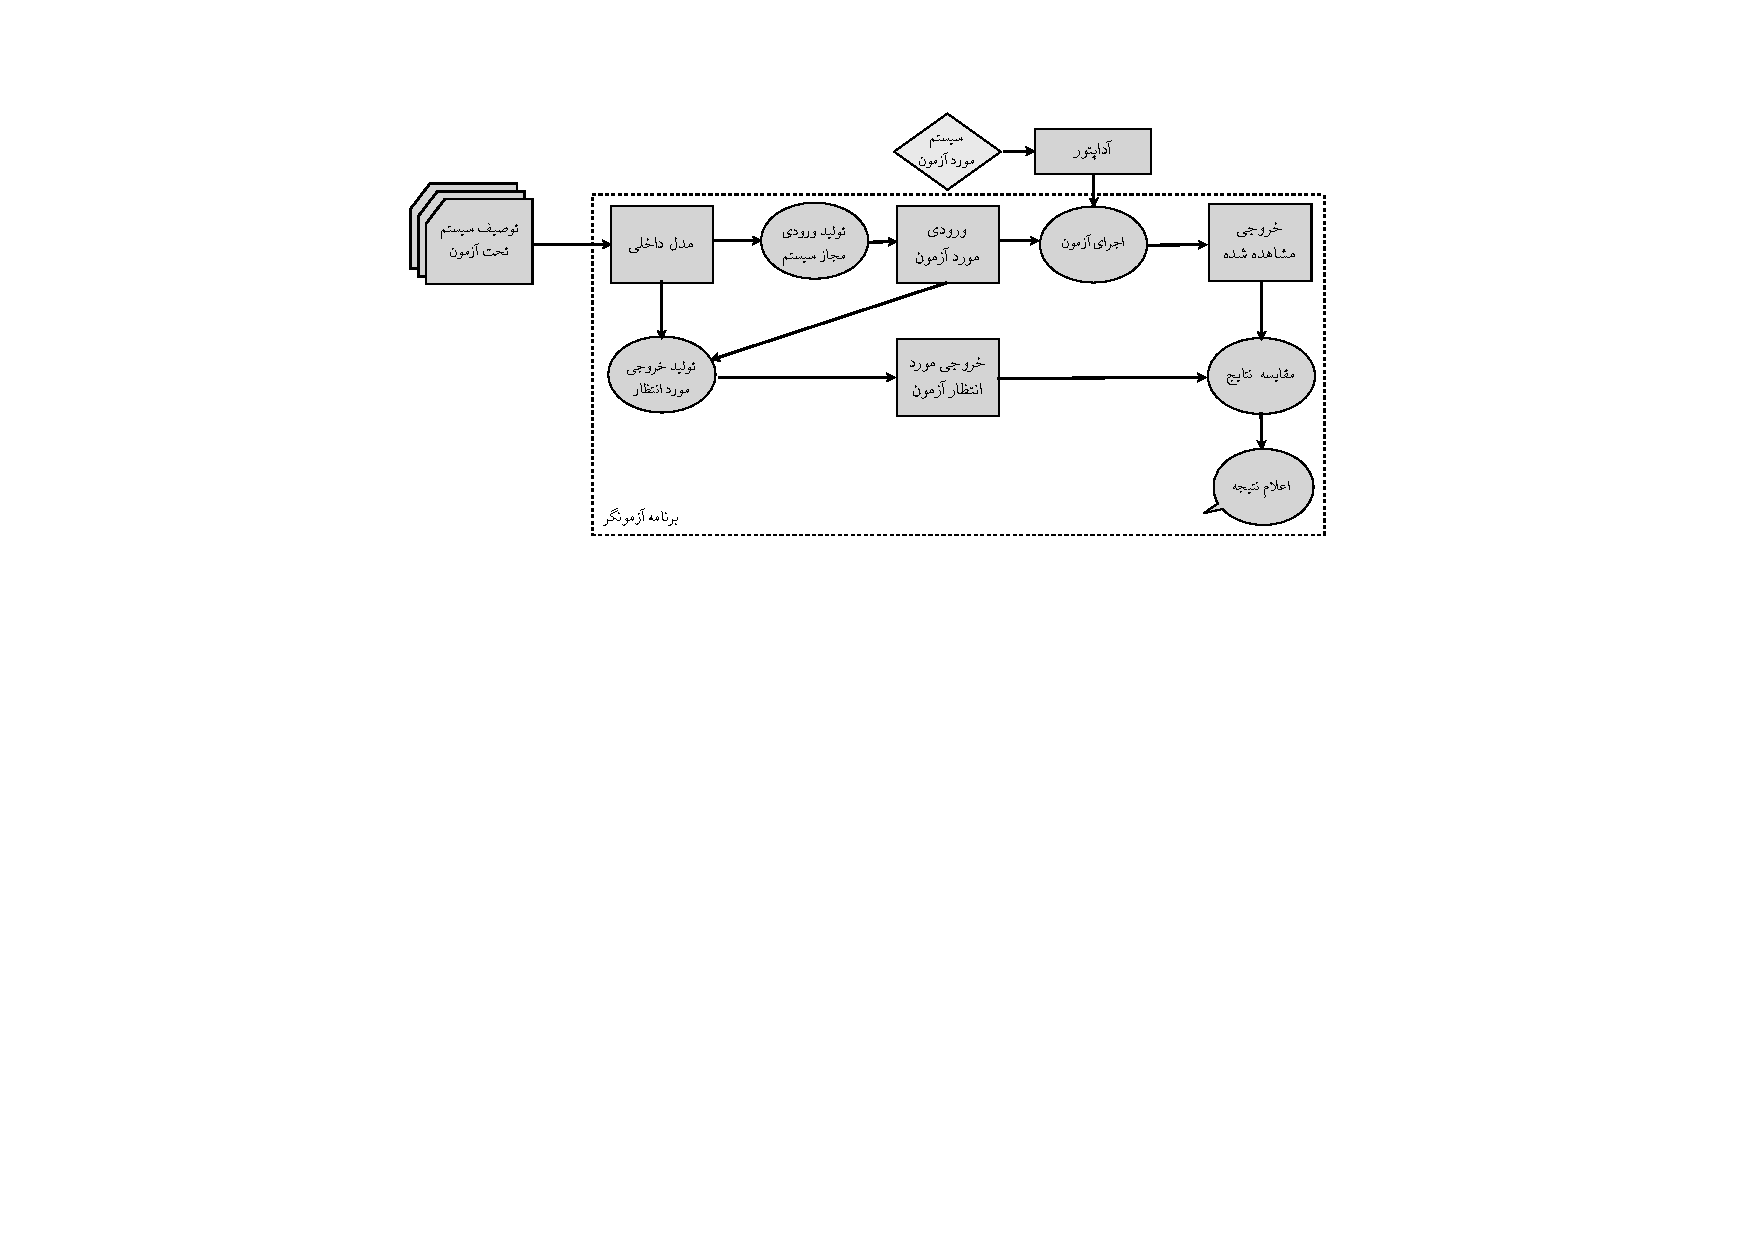
\includegraphics[width=11cm]{2-Preliminaries/Figures/mbtOverview.pdf}
	\\
	\hline
  \end{tabular}
  \end{center}
   \caption{\label{fig:mbtOverview} نمای سطح بالای مراحل آزمون در روش مبتنی بر مدل \cite{utting06}}
\end{figure}


\section{ساختار پایان‌نامه}
برای بررسی این موارد، ساختار این متن در ۶ فصل تنظیم گردیده است:
\begin{strict_itemize}
\item
 فصل \ref{chapter:Preliminaries} به بررسی برخی پیش‌نیازهای تعریف چهارچوب پیشنهادی می‌پردازد. رابطه‌ی مطابقت آی‌اوکو و روش افراز رده‌ای در این بخش به طور خلاصه مورد بررسی قرار گرفته‌اند.
\item
در فصل \ref{chapter:RelatedWork} برخی از کارهای قبلی و مرتبط با مسئله‌ی آزمون مبتنی بر مدل و راه‌حل‌های آن معرفی شده‌اند. هم‌چنین بعضی از مهم‌ترین ابزارهای آزمون نرم‌افزار که مبتنی بر مدل نیستند اما پشتیبانی خوبی برای آزمون سیستم‌های مبتنی بر داده دارند نیز بررسی شده‌اند. 
\item
فصل \ref{chapter:proposedFramework} ایده‌ی پیشنهادی در این پژوهش به طور مبسوط مورد بحث قرار داده است. این ایده (آن‌چنان که پیش از این نیز اشاره شد) عبارت از ارائه‌ی یک چهارچوب برای آزمون مبتنی بر مدل سیستم‌هایی است که هم از حیث رفتاری و هم از تاثیرپذیری از مقادیر داده‌ای که مبادله می‌کنند، پیچیده‌اند. در این فصل هم به نحو و هم به معنای این چهارچوب پرداخته شده است. برای نحو چهارچوب پیشنهادی از زبان یو‌ام‌ال استفاده شده است و معنای آن نیز بر روش آی‌اوکو (که در فصل \ref{chapter:Preliminaries} مورد بررسی قرار می‌گیرد) استوار است.
\item
 در فصل \ref{chapter:caseStudy} یک مطالعه‌ی موردی از آزمون یک سیستم واقعی از حوزه‌ی نرم‌افزارهای مالی، با استفاده از روش پیشنهادی، مورد بررسی قرار خواهد گرفت. برای این منظور معیاری عددی برای مقایسه‌ی آزمون‌های تولید شده توسط این چهارچوب و آزمون‌های تولید شده توسط روش‌های دیگر ارائه شده و نتایج حاصله تحلیل شده‌اند.
\item
نهایتاً فصل \ref{chapter:Conclusion} برخی نکات پایانی را مطرح و در مورد جهت‌گیری‌های احتمالی آینده‌ی این پژوهش مطالبی ارائه می‌کند.
\end{strict_itemize}